\documentclass[tikz,border=6pt]{standalone}
\usepackage{amsmath,amssymb}
\definecolor{inD}{RGB}{31,94,165}\definecolor{inC}{RGB}{214,96,33}
\tikzset{
  m/.style={circle,inner sep=0pt,minimum size=9pt,ball color=inD!85,draw=inD!60!black,line width=0.3pt},
  c/.style={circle,inner sep=0pt,minimum size=9pt,ball color=inC!90,draw=inC!60!black,line width=0.3pt},
  lab/.style={font=\small,fill=white,fill opacity=0.85,text opacity=1,inner sep=1.2pt,rounded corners=1pt},
  e/.style={line width=0.75pt,black!55},
  ec/.style={line width=1.4pt,inC!80!black},
  ex/.style={line width=0.6pt,black!35,densely dashed}}
\begin{document}

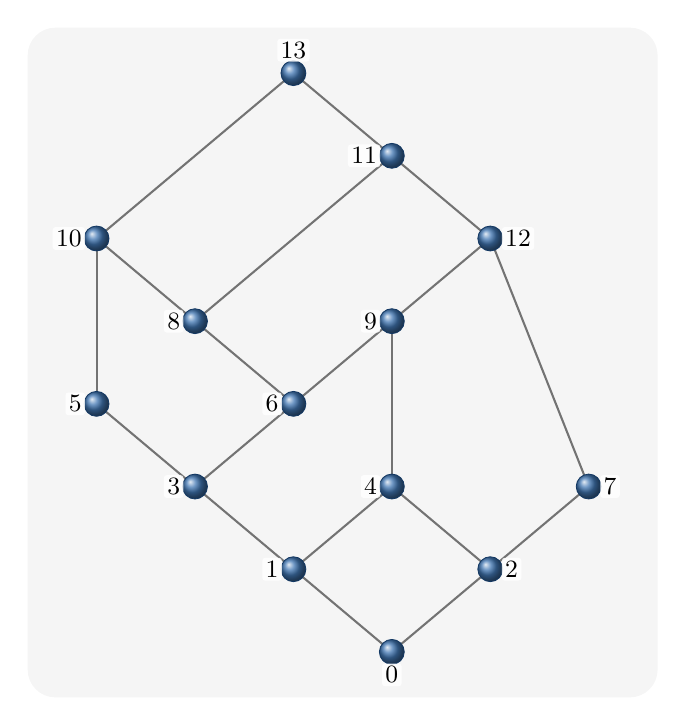
\begin{tikzpicture}[x=1.25cm,y=1.05cm]
\fill[black!4,rounded corners=10pt] (-3.7,-0.55) rectangle (2.7,7.55);
\coordinate (k0) at (0,0);
\coordinate (k1) at (-1,1);
\coordinate (k2) at (1,1);
\coordinate (k3) at (-2,2);
\coordinate (k4) at (0,2);
\coordinate (k7) at (2,2);
\coordinate (k5) at (-3,3);
\coordinate (k6) at (-1,3);
\coordinate (k8) at (-2,4);
\coordinate (k9) at (0,4);
\coordinate (k10) at (-3,5);
\coordinate (k12) at (1,5);
\coordinate (k11) at (0,6);
\coordinate (k13) at (-1,7);
\draw[e] (k0) -- (k1);
\draw[e] (k0) -- (k2);
\draw[e] (k1) -- (k3);
\draw[e] (k1) -- (k4);
\draw[e] (k2) -- (k4);
\draw[e] (k2) -- (k7);
\draw[e] (k3) -- (k5);
\draw[e] (k3) -- (k6);
\draw[e] (k4) -- (k9);
\draw[e] (k5) -- (k10);
\draw[e] (k6) -- (k8);
\draw[e] (k6) -- (k9);
\draw[e] (k7) -- (k12);
\draw[e] (k8) -- (k10);
\draw[e] (k8) -- (k11);
\draw[e] (k9) -- (k12);
\draw[e] (k10) -- (k13);
\draw[e] (k11) -- (k13);
\draw[e] (k12) -- (k11);
\node[m] at (k0) {}; \node[lab,below=4pt] at (k0) {$0$};
\node[m] at (k1) {}; \node[lab,left=4pt] at (k1) {$1$};
\node[m] at (k2) {}; \node[lab,right=4pt] at (k2) {$2$};
\node[m] at (k3) {}; \node[lab,left=4pt] at (k3) {$3$};
\node[m] at (k4) {}; \node[lab,left=4pt] at (k4) {$4$};
\node[m] at (k7) {}; \node[lab,right=4pt] at (k7) {$7$};
\node[m] at (k5) {}; \node[lab,left=4pt] at (k5) {$5$};
\node[m] at (k6) {}; \node[lab,left=4pt] at (k6) {$6$};
\node[m] at (k8) {}; \node[lab,left=4pt] at (k8) {$8$};
\node[m] at (k9) {}; \node[lab,left=4pt] at (k9) {$9$};
\node[m] at (k10) {}; \node[lab,left=4pt] at (k10) {$10$};
\node[m] at (k12) {}; \node[lab,right=4pt] at (k12) {$12$};
\node[m] at (k11) {}; \node[lab,left=4pt] at (k11) {$11$};
\node[m] at (k13) {}; \node[lab,above=4pt] at (k13) {$13$};
\end{tikzpicture}
\end{document}
